\chapter{System Requirements and Methodology}

\section{Introduction}
The primary objective of this project is to develop, rigorously benchmark, and clinically evaluate an end-to-end deep learning framework for synthetic CT (sCT) generation from magnetic resonance imaging (MRI). To ensure reproducibility and clinical relevance, the methodology strictly adheres to the protocols established by the international SynthRAD2023 Grand Challenge~\cite{thummerer2023synthrad2023}. 

This chapter delineates the hardware and software specifications, dataset cohort stratification, intensity calibration pipelines, Data Flow Diagrams (DFDs), comprehensive mathematical architectures of the five evaluated generative models, and the multi-dimensional quantitative evaluation framework.

\section{System Requirements Specifications (SRS)}

\subsection{Hardware Requirements}
Deep generative models—particularly iterative diffusion frameworks—impose rigorous computational demands during training and inference. The minimum and recommended hardware specifications utilized in this benchmark are outlined in Table~\ref{tab:hardware_req}.

\begin{table}[htbp]
\centering
\caption{System Hardware Requirements for Training and Benchmarking}
\label{tab:hardware_req}
\small
\renewcommand{\arraystretch}{1.3}
\begin{tabularx}{\textwidth}{@{} l p{5.5cm} X @{}}
\toprule
\textbf{Component} & \textbf{Minimum Specification} & \textbf{Benchmarked Environment} \\
\midrule
Graphics Processing Unit (GPU) & NVIDIA RTX 3060 (12 GB VRAM) & NVIDIA Tesla T4 / RTX 4090 (16--24 GB VRAM) \\
CUDA Compute Capability & Version 7.5+ & Version 8.0+ / 8.9 (Tensor Cores enabled) \\
Host Processor (CPU) & Intel Core i7 / AMD Ryzen 7 (8 Cores) & Intel Xeon / AMD EPYC (16 vCPUs) \\
Host System RAM & 16 GB DDR4 & 32 GB DDR4 / DDR5 ECC \\
Storage Medium & 100 GB SATA SSD & 512 GB High-Speed NVMe PCIe 4.0 SSD \\
Display & Full HD ($1920 \times 1080$) & $4\text{K UHD } (3840 \times 2160)$ Diagnostic Monitor \\
\bottomrule
\end{tabularx}
\end{table}

\subsection{Software Requirements and Environment Stack}
The complete software architecture is constructed on open-source, reproducible deep learning frameworks running in modern CUDA environments. Table~\ref{tab:software_req} specifies the software stack.

\begin{table}[htbp]
\centering
\caption{System Software Stack and Dependent Frameworks}
\label{tab:software_req}
\small
\renewcommand{\arraystretch}{1.3}
\begin{tabularx}{\textwidth}{@{} l p{4.5cm} X @{}}
\toprule
\textbf{Software Layer} & \textbf{Package / Tool} & \textbf{Version \& Purpose} \\
\midrule
Operating System & Microsoft Windows 11 / Linux Ubuntu & 64-bit OS with CUDA kernel support \\
Core Language & Python & Version 3.10.12 (CPython runtime) \\
Deep Learning Framework & PyTorch & Version 2.2.0+cu121 (Autograd engine) \\
Vision Toolkits & Torchvision, OpenCV & Image transforms, tensor manipulation \\
Medical Image I/O & SimpleITK, Nibabel & Reading NIfTI, DICOM, and HU header tags \\
Scientific Computing & NumPy, SciPy & High-performance array operations \\
Visualization \& Plotting & Matplotlib, Seaborn & Residual difference maps and distribution plots \\
Model Compilation & TorchScript / CUDA Graphs & Accelerated inference runtime \\
\bottomrule
\end{tabularx}
\end{table}

\section{Dataset Architecture and Preprocessing Pipeline}

\subsection{SynthRAD2023 Grand Challenge Brain Dataset}
The models are evaluated on the public SynthRAD2023 Grand Challenge cranial dataset~\cite{thummerer2023synthrad2023}. The cohort comprises high-resolution paired $T_1$-weighted Magnetic Resonance Imaging (MRI) and corresponding Computed Tomography (CT) scans acquired from multi-institutional clinical radiotherapy centers. All volumetric acquisitions undergo rigid skull-base coregistration and reslicing to an isotropic spatial resolution of $1.0 \times 1.0 \times 1.0\text{ mm}^3$ with standard $256 \times 256$ in-plane slice matrix dimensions.

\subsection{Data Leakage Prevention and Cohort Splitting}
To guarantee rigorous statistical independence and prevent inter-slice data leakage between training and testing distributions:
\begin{itemize}
    \item All data splits are performed strictly at the **patient cohort level** rather than random slice-wise mixing.
    \item An $80\% / 20\%$ stratified patient-level partitioning is executed under a deterministic random seed ($\text{Seed} = 42$).
    \item The held-out test cohort comprises exactly 363 axial paired 2D slices spanning all cranial levels, from the posterior cranial fossa and skull base through the ventricular system to the superior vertex.
\end{itemize}

\subsection{Intensity Calibration and Physical Hounsfield Unit Scaling}
CT voxel values represent physical Hounsfield Units (HU) governed by tissue attenuation coefficients. To prepare raw CT volumes for stable neural network training while preserving clinical range validity, voxel values are bounded within the standard cranial radiotherapy window $[-1000\text{ HU}, +3000\text{ HU}]$ and mapped to the normalized neural dynamic range $[-1.0, +1.0]$:
\begin{equation}
y_{\text{norm}} = 2 \times \left( \frac{y_{\text{HU}} - \text{HU}_{\min}}{\text{HU}_{\max} - \text{HU}_{\min}} \right) - 1.0
\label{eq:ct_norm_forward}
\end{equation}
where $\text{HU}_{\min} = -1000\text{ HU}$ (air attenuation) and $\text{HU}_{\max} = +3000\text{ HU}$ (dense dense cortical skull bone).

During inference and metric evaluation, predicted synthetic CT tensors $\mathbf{\hat{y}}_{\text{norm}} \in [-1.0, +1.0]$ are deterministically inverted back to true physical Hounsfield Units:
\begin{equation}
\hat{y}_{\text{HU}} = \left( \frac{\mathbf{\hat{y}}_{\text{norm}} + 1.0}{2.0} \right) \times (\text{HU}_{\max} - \text{HU}_{\min}) + \text{HU}_{\min}
\label{eq:ct_norm_inverse}
\end{equation}

Similarly, input MRI slices are normalized to $[-1.0, +1.0]$ using min-max scaling computed within the non-zero brain mask region to eliminate background radiofrequency noise bias.

\section{System Architecture and Data Flow Diagrams (DFD)}

\subsection{DFD Level 0: Context Level Diagram}
Figure~\ref{fig:dfd_0} depicts the Level 0 Context Diagram of the proposed MRI-to-CT translation system. The clinical user (Radiation Oncologist / Medical Physicist) supplies raw $T_1$-weighted MR acquisitions, and the automated system returns a geometrically aligned, calibrated Synthetic CT (sCT) volume along with clinical dosimetric confidence reports.

\begin{figure}[htbp]
\centering
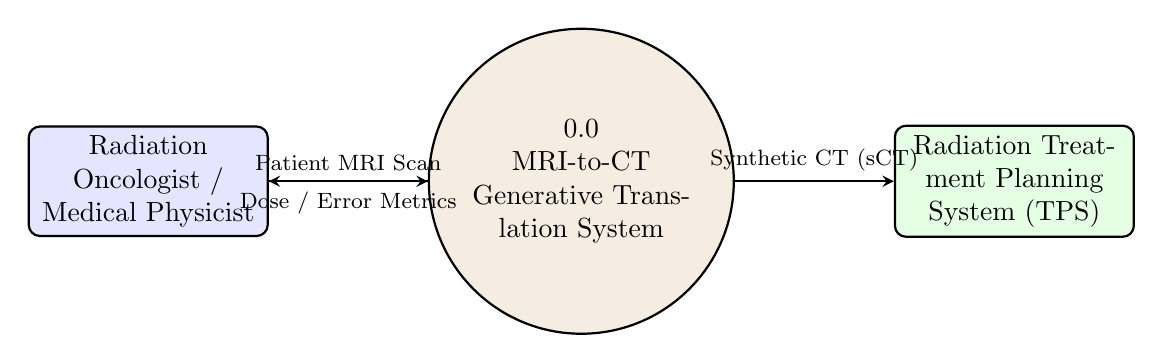
\begin{tikzpicture}[node distance=3cm, auto, >=stealth, thick]
  \node [draw, rectangle, rounded corners, fill=blue!10, text width=2.8cm, text centered, minimum height=1.2cm] (user) {Radiation Oncologist / Medical Physicist};
  \node [draw, circle, fill=brown!15, text width=3.2cm, text centered, minimum height=3.2cm, right of=user, node distance=5.5cm] (system) {0.0\\MRI-to-CT\\Generative Translation System};
  \node [draw, rectangle, rounded corners, fill=green!10, text width=2.8cm, text centered, minimum height=1.2cm, right of=system, node distance=5.5cm] (tps) {Radiation Treatment Planning System (TPS)};

  \draw [->] (user) -- node[above, font=\footnotesize] {Patient MRI Scan} (system);
  \draw [->] (system) -- node[above, font=\footnotesize] {Synthetic CT (sCT)} (tps);
  \draw [->] (system) -- node[below, font=\footnotesize] {Dose / Error Metrics} (user);
\end{tikzpicture}
\caption{DFD Level 0: Context-Level Interaction Diagram}
\label{fig:dfd_0}
\end{figure}

\subsection{DFD Level 1: Core Processing Pipeline}
Figure~\ref{fig:dfd_1} illustrates the operational Level 1 decomposition:
\begin{enumerate}
    \item \textbf{Process 1.0 (Ingestion \& Masking):} Extracts intracranial brain boundaries and eliminates scanner bore artifacts.
    \item \textbf{Process 2.0 (Physical Scaling):} Applies dynamic range normalization to $[-1.0, 1.0]$.
    \item \textbf{Process 3.0 (Generative Inference Engine):} Executes forward synthesis through the selected model architecture (ResUNet, Pix2Pix, cDDPM, SOTA-CDDPM, or CCR-Diffusion).
    \item \textbf{Process 4.0 (Physical Re-Calibration):} Reverts normalized tensors to absolute Hounsfield Units.
    \item \textbf{Process 5.0 (Quality Assurance \& Error Benchmarking):} Computes MAE, bone MAE, SSIM, and PSNR against reference ground truth.
\end{enumerate}

\begin{figure}[htbp]
\centering
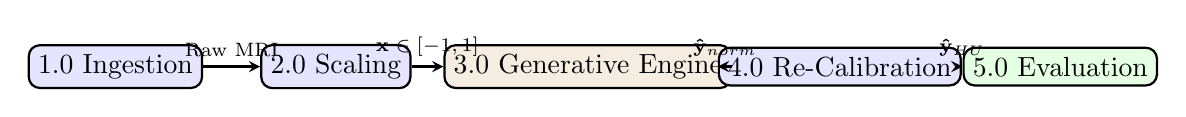
\begin{tikzpicture}[node distance=2.2cm, auto, >=stealth, thick]
  \node [draw, rectangle, rounded corners, fill=blue!10, minimum width=2.2cm] (p1) {1.0 Ingestion};
  \node [draw, rectangle, rounded corners, fill=blue!10, right of=p1, node distance=2.8cm] (p2) {2.0 Scaling};
  \node [draw, rectangle, rounded corners, fill=brown!15, right of=p2, node distance=3.2cm] (p3) {3.0 Generative Engine};
  \node [draw, rectangle, rounded corners, fill=blue!10, right of=p3, node distance=3.2cm] (p4) {4.0 Re-Calibration};
  \node [draw, rectangle, rounded corners, fill=green!10, right of=p4, node distance=2.8cm] (p5) {5.0 Evaluation};

  \draw [->] (p1) -- node[above, font=\scriptsize] {Raw MRI} (p2);
  \draw [->] (p2) -- node[above, font=\scriptsize] {$\mathbf{x} \in [-1, 1]$} (p3);
  \draw [->] (p3) -- node[above, font=\scriptsize] {$\mathbf{\hat{y}}_{\text{norm}}$} (p4);
  \draw [->] (p4) -- node[above, font=\scriptsize] {$\mathbf{\hat{y}}_{\text{HU}}$} (p5);
\end{tikzpicture}
\caption{DFD Level 1: Subsystem Data Flow Architecture}
\label{fig:dfd_1}
\end{figure}

\subsection{DFD Level 2: Generative Reverse Diffusion Sampling Process}
Figure~\ref{fig:dfd_2} specifies the internal reverse Langevin / DDIM loop (Process 3.0) governing Models 3, 4, and 5.

\begin{figure}[htbp]
\centering
\begin{tikzpicture}[node distance=1.8cm, auto, >=stealth, thick]
  \node [draw, ellipse, fill=gray!20] (noise) {Gaussian Noise $\mathbf{y}_T \sim \mathcal{N}(\mathbf{0}, \mathbf{I})$};
  \node [draw, rectangle, fill=brown!10, below of=noise] (step) {Time Step $t = \tau_i$};
  \node [draw, rectangle, rounded corners, fill=blue!10, below of=step] (denoiser) {Denoiser $\boldsymbol{\epsilon}_\theta(\mathbf{y}_t, t, \mathbf{x}, \mathbf{m})$};
  \node [draw, rectangle, fill=yellow!15, below of=denoiser] (update) {DDIM Update $\mathbf{y}_{\tau_{i-1}}$};
  \node [draw, diamond, aspect=2, fill=purple!10, below of=update, node distance=2.2cm] (check) {$i = 1$?};
  \node [draw, rectangle, rounded corners, fill=green!15, right of=check, node distance=4.5cm] (out) {Synthesized CT $\mathbf{y}_0$};

  \draw [->] (noise) -- (step);
  \draw [->] (step) -- (denoiser);
  \draw [->] (denoiser) -- (update);
  \draw [->] (update) -- (check);
  \draw [->] (check) -- node[above, font=\footnotesize] {Yes} (out);
  \draw [->] (check.west) -- ++(-1.0, 0) |- node[near start, left, font=\footnotesize] {No ($i \leftarrow i-1$)} (step.west);
\end{tikzpicture}
\caption{DFD Level 2: DDIM 50-Step Deterministic Reverse Sampling Loop}
\label{fig:dfd_2}
\end{figure}

\section{Detailed Architectural Design of the Five Evaluated Models}

\subsection{Model 1: Deep Residual U-Net (ResUNet Baseline)}
Model 1 provides a direct supervised convolutional regression baseline~\cite{zhang2018road}. The network employs a 4-level encoder-decoder hierarchy:
\begin{itemize}
    \item \textbf{Residual Encoder:} Consists of stacked residual units where each block comprises two $3\times3$ convolutions with Group Normalization (16 groups) and GELU activations, bypassed by an identity $1\times1$ projection shortcut. The feature channel dimensions expand sequentially: $64 \to 128 \to 256 \to 512$.
    \item \textbf{Bottleneck:} Two cascading residual blocks operating at spatial resolution $16 \times 16$ with 512 channels.
    \item \textbf{Residual Decoder:} Bilinear upsampling followed by channel concatenation with skip connections and residual convolutions ($512 \to 256 \to 128 \to 64$).
    \item \textbf{Objective Function:} A composite $L_1$ and Mean Squared Error loss:
    \begin{equation}
    \mathcal{L}_{\text{M1}}(\theta) = \frac{1}{|\Omega|} \sum_{i \in \Omega} |\hat{y}_i - y_i| + 0.1 \cdot \frac{1}{|\Omega|} \sum_{i \in \Omega} (\hat{y}_i - y_i)^2
    \label{eq:m1_detailed_loss}
    \end{equation}
\end{itemize}

\subsection{Model 2: Conditional GAN (Pix2Pix)}
Model 2 adapts conditional adversarial translation~\cite{isola2017image,nie2017medical}.
\begin{itemize}
    \item \textbf{Generator ($G$):} A U-Net topology with skip connections mapping $\mathbf{x} \to \mathbf{\hat{y}}$.
    \item \textbf{Discriminator ($D$):} A $70 \times 70$ PatchGAN evaluating 2-channel concatenated pairs $[\mathbf{x} \mathbin{\Vert} \mathbf{y}]$.
    \item \textbf{Adversarial Formulation:}
    \begin{equation}
    \min_G \max_D \mathbb{E}_{\mathbf{x}, \mathbf{y}}[\log D(\mathbf{x}, \mathbf{y})] + \mathbb{E}_{\mathbf{x}}[\log(1 - D(\mathbf{x}, G(\mathbf{x})))] + 100 \cdot \|\mathbf{y} - G(\mathbf{x})\|_1
    \label{eq:m2_detailed_loss}
    \end{equation}
\end{itemize}

\subsection{Model 3: Conditional DDPM From Scratch}
Model 3 trains an unconstrained conditional diffusion model directly on paired SynthRAD2023 data~\cite{ho2020denoising,saharia2022palette}.
\begin{itemize}
    \item \textbf{Noise Schedule:} 1000-step linear schedule with $\beta_1 = 10^{-4}$ and $\beta_T = 0.02$.
    \item \textbf{Input Conditioning:} Early concatenation of 3 channels: $[\mathbf{y}_t \mathbin{\Vert} \mathbf{x} \mathbin{\Vert} \mathbf{m}]$.
    \item \textbf{Denoiser Architecture:} Time-embedded U-Net with sinusoidal timestep embeddings projected through 2-layer MLPs to all intermediate feature blocks.
    \item \textbf{Inference:} Accelerated DDIM sampling ($S = 50$ steps, $\eta = 0$).
\end{itemize}

\subsection{Model 4: SOTA-CDDPM with Residual Attention and Bone Loss}
Model 4 enhances conditional diffusion through self-attention gating and targeted anatomical loss shaping~\cite{kazerouni2023diffusion}.
\begin{itemize}
    \item \textbf{Cross-Layer Attention Gates:} Placed at the skip connections between encoder and decoder to filter spatial background noise:
    \begin{equation}
    \alpha_{i,j} = \sigma\left( \psi^T \left[ \text{ReLU}(W_g \mathbf{g}_{i,j} + W_x \mathbf{x}_{i,j} + b_g) \right] + b_\psi \right)
    \label{eq:att_gate}
    \end{equation}
    \item \textbf{Bone-Weighted Hybrid Loss:} Quadruples penalty on high-density cortical structures:
    \begin{equation}
    \mathcal{L}_{\text{M4}} = \|\boldsymbol{\epsilon} - \hat{\boldsymbol{\epsilon}}\|_2^2 + 2.0 \cdot \mathbb{E}[\mathbf{w}_{\text{bone}} \odot |\mathbf{\hat{y}}_0 - \mathbf{y}_0|] + 0.5 \cdot (1 - \text{SSIM}(\mathbf{\hat{y}}_0, \mathbf{y}_0))
    \label{eq:m4_bone_loss}
    \end{equation}
    where $\mathbf{w}_{\text{bone}} = 1.0 + 4.0 \cdot \mathbb{I}(y_{\text{real}} > 300\text{ HU})$.
\end{itemize}

\subsection{Model 5: Proposed Cross-Conditioned Residual Diffusion (CCR-Diffusion)}
Model 5 introduces a novel two-stage decoupled architecture designed to eliminate diffusion drift while preserving fine bone calcification fidelity.
\begin{enumerate}
    \item \textbf{Stage 1 (Coarse Anatomical Anchor):} A deterministic residual network generates coarse approximation $\mathbf{c} = f_{\text{stage1}}(\mathbf{x}) \in [-1.0, 1.0]$. Multi-scale feature tensors $\mathbf{F}_{\text{enc}}^{(l)}$ are extracted at 4 hierarchical depths.
    \item \textbf{Stage 2 (FiLM-Modulated Residual Diffusion):} The diffusion denoiser models only the standardized residual:
    \begin{equation}
    \mathbf{z}_0 = \frac{\mathbf{y} - \mathbf{c}}{s}, \quad \text{where } s = \sigma(\mathbf{y} - \mathbf{c})
    \label{eq:res_std}
    \end{equation}
    At each decoder stage, Feature-wise Linear Modulation (FiLM) dynamically modulates features:
    \begin{equation}
    \text{FiLM}(\mathbf{F}; \boldsymbol{\gamma}, \boldsymbol{\beta}) = (1.0 + \boldsymbol{\gamma}) \odot \mathbf{F} + \boldsymbol{\beta}
    \label{eq:film_layer}
    \end{equation}
    Reconstruction is achieved deterministically:
    \begin{equation}
    \mathbf{\hat{y}} = \text{clip}(\mathbf{c} + s \cdot \mathbf{z}_0, \; -1.0, \; 1.0)
    \label{eq:ccr_final_recon}
    \end{equation}
\end{enumerate}

\section{Evaluation Framework and Clinical Metrics}
Each synthesized volume is evaluated across four primary clinical and quantitative criteria:
\begin{enumerate}[label=\textbf{(\arabic*)}]
    \item \textbf{Global Mean Absolute Error ($\text{MAE}_{\text{all}}$):} Computed across all intracranial voxels within the non-zero brain mask $\Omega$:
    \begin{equation}
    \text{MAE}_{\text{all}} = \frac{1}{|\Omega|} \sum_{i \in \Omega} |\hat{y}_{\text{HU}, i} - y_{\text{HU}, i}|
    \label{eq:mae_all}
    \end{equation}
    \item \textbf{Bone-Specific Mean Absolute Error ($\text{MAE}_{\text{bone}}$):} Evaluated specifically over cortical bone voxels ($\Omega_{\text{bone}} = \{i \in \Omega \mid y_{\text{HU}, i} > 300\text{ HU}\}$):
    \begin{equation}
    \text{MAE}_{\text{bone}} = \frac{1}{|\Omega_{\text{bone}}|} \sum_{i \in \Omega_{\text{bone}}} |\hat{y}_{\text{HU}, i} - y_{\text{HU}, i}|
    \label{eq:mae_bone}
    \end{equation}
    \item \textbf{Structural Similarity Index Measure (SSIM):} Quantifies perceptual luminance, contrast, and structural degradation~\cite{wang2004image}:
    \begin{equation}
    \text{SSIM}(\mathbf{x}, \mathbf{y}) = \frac{(2\mu_x\mu_y + C_1)(2\sigma_{xy} + C_2)}{(\mu_x^2 + \mu_y^2 + C_1)(\sigma_x^2 + \sigma_y^2 + C_2)}
    \label{eq:ssim_metric}
    \end{equation}
    \item \textbf{Peak Signal-to-Noise Ratio (PSNR):} Measures logarithmic signal fidelity:
    \begin{equation}
    \text{PSNR} = 10 \cdot \log_{10} \left( \frac{\text{MAX}^2}{\text{MSE}} \right), \quad \text{MAX} = 4000\text{ HU}
    \label{eq:psnr_metric}
    \end{equation}
    \item \textbf{Computational Efficiency Profiling:} Inference latency (milliseconds per slice), throughput (frames per second, FPS), total parameters, trainable parameters, and peak GPU VRAM allocation.
\end{enumerate}
